\subsection{Approach}
\label{sec:soft_cut_approach}

For the soft cut detection we decided to use a deep learning approach.
More concrete we used the RNN/LSTM implementation by Jeff Donahue\footnote{\url{https://github.com/BVLC/caffe/pull/2033}}. \\
This RNN/LSTM implementation takes two different inputs: On the one hand the raw pixel values and on the other hand a tagging sequence.
A tagging seuqence represents sequences of frames, where one sequence of frames might represent a soft cut in our case.
Using this implementation allows us to incorporate the information of a frame, which is at the beginning of a frame sequence, to a frame, which is located later in the same sequence.
So the net memorizes previous decision along a sequence of frames. \\
But using this architecture has one problem, as stated by Jeff Donahue: `"backpropagation [through the LSTM] is truncated along the batch boundaries'" [TODO: Quelle].
So one or more frame sequences has to fit exactly into the batch size used by the RNN/LSTM.
This is hard to archive if we want to use variable length of frame sequences.
Therefore we decided to use a fixed size for the sequences of frames in a tagging sequence, i.e. we only check for example 10 consecutive frames of being a soft cut or not.  \\
However, we still want to find soft cut of arbitrary length in a video.
To achieve this, we repeatedly test fixed-size frame sequences.
In Figure~\ref{fig:soft_cut_approach} an example is shown.

\begin{figure}[!htb]
	\centering
	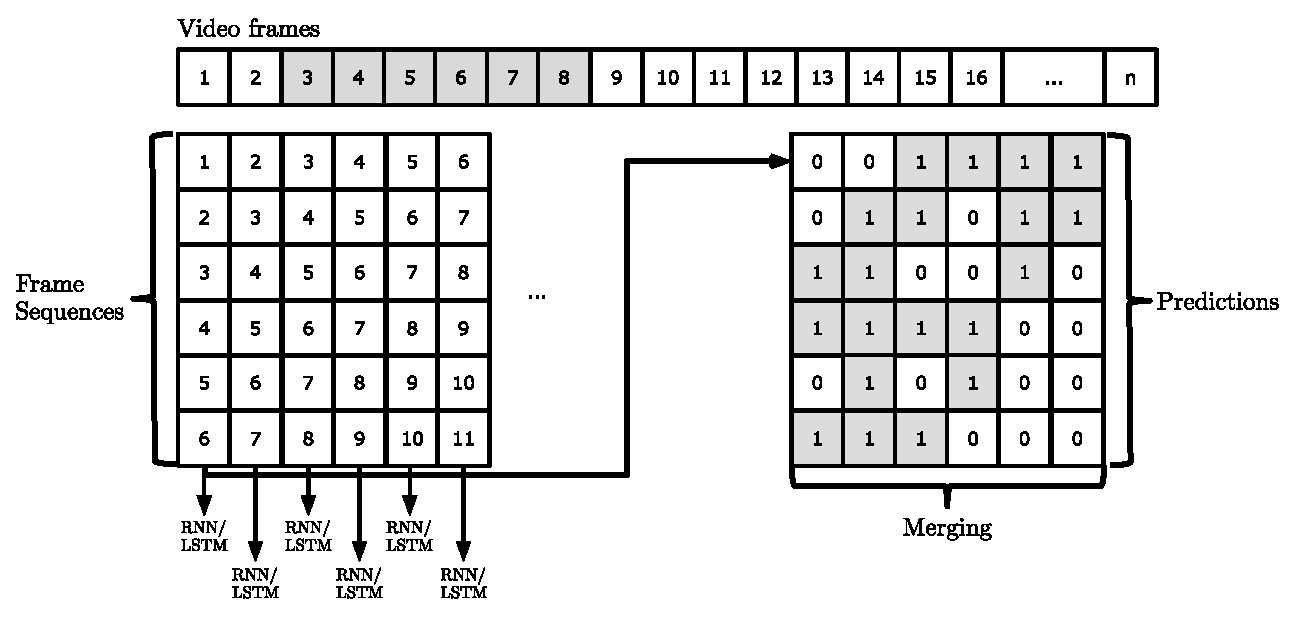
\includegraphics[scale=.7]{images/soft_cut_approach.eps}
	\caption{To classify soft cuts of arbitrary length, we repeatedly test fixed-size frame sequences. In this example we test sequences of size six. Afterwards the predictions given by the RNN/LSTM are merged, so that we have one prediction per frame.}
	\label{fig:soft_cut_approach}
\end{figure}

We have a video with \textit{n} frames.
The frames from three to eight represent a soft cut.
We now generated for each frame a frame sequence of size six.
Those sequences are then classified by the RNN/LSTM.
The output of the RNN/LSTM is zero, if a frame does not belong to a soft cut, and one, otherwise.
In the end we have up six prediction per frame, which have to be merged, so that we only have one prediction per frame.
After the merging step consecutive frames, which got a prediction of one, i.e. the frame is part of an soft cut, represent a soft cut. \\
In the following several strategies for combining the multiple frame prediction into one prediction are presented.

\subsubsection{Take First}
\subsubsection{Take Last 'Sequence'}
\subsubsection{Take Last 'Frame'}
\subsubsection{Majority-Voting Diagonally}
